\phantomsection
\addcontentsline{toc}{section}{Apuntes}
\begin{center}
\end{center}

\phantomsection
\addcontentsline{toc}{subsection}{Unidad 1. Introducción}
\subsection*{\textcolor{blueunam}{Unidad 1. Introducción}}

\begin{notadidactica}
\textbf{Sobre las notas en este documento.} Hay tres niveles según su importancia:

\begin{itemize}
    \item \textcolor{rojoNota}{\textbf{Notas relevantes}} (línea roja gruesa): 
    convenciones, definiciones y sistemas de notación que se usan en todo el 
    documento. No se pueden ignorar.
    \item \textcolor{amarilloNota}{\textbf{Notas importantes}} (línea amarilla 
    media): aclaraciones conceptuales, justificaciones y puentes entre ideas. 
    Opcionales, pero recomendadas.
    \item \textcolor{azulNota}{\textbf{Notas didácticas}} (línea azul delgada): 
    analogías, ejemplos cotidianos e intuiciones. Totalmente opcionales.
\end{itemize}
\end{notadidactica}

\begin{notaimportante}
\textbf{Conocimientos previos recomendados.} Este curso asume familiaridad con:

\begin{itemize}
    \item \textbf{Álgebra:} despeje de variables, resolución de sistemas 
    de dos o tres ecuaciones lineales, factorización básica.
    \item \textbf{Cálculo:} derivadas e integrales elementales, regla de 
    la cadena, integración por partes. No se derivan aquí.
    \item \textbf{Química general:} masa molar, estequiometría, 
    concentraciones, gases ideales.
    \item \textbf{Herramientas de cómputo:} Excel o LibreOffice Calc para 
    tablas y cálculos repetitivos; draw.io o Inkscape para diagramas de flujo.
\end{itemize}

Si alguna de estas áreas genera dificultad, no es un bloqueo para el curso,
pero conviene repasarla conforme aparezca. Los apuntes no cubren los
fundamentos de estas herramientas; se asumen.
\end{notaimportante}

% ══════════════════════════════════════════════════════════════
%  CLASE 1
% ══════════════════════════════════════════════════════════════

\phantomsection
\addcontentsline{toc}{subsubsection}{Clase 1 -- 19/08/2026: Unidades y factores de conversión}
\subsubsection*{\textcolor{blueunam}{Clase 1 -- 19/08/2026: Unidades y factores de conversión}}

\textbf{Magnitud física:} propiedad medible de un sistema que se puede
expresar como un número acompañado de una unidad. Sin unidad, un número
no dice nada: decir ``la tubería mide 5'' no informa nada; decir
``la tubería mide $5\,\mathrm{m}$'' sí.

Toda cantidad física se escribe como
\[
\text{cantidad} = \text{número} \times \text{unidad}
\]
Omitir la unidad en un resultado es un error de comunicación, no un
detalle estético. En ingeniería y cualquier disciplina, una cifra sin unidad se considera
incompleta.

\textbf{Sistema Internacional de Unidades (SI).} Es el sistema de
referencia. Tiene siete unidades base, de las cuales en este curso se
usan las primeras cinco:

\begin{center}
\renewcommand{\arraystretch}{1.4}
\begin{tabular}{|L{3cm}|L{2.5cm}|L{3cm}|L{4cm}|}
\hline
\textbf{Magnitud} & \textbf{Símbolo} & \textbf{Unidad SI} & \textbf{Símbolo} \\
\hline
Longitud & $L$ & metro & $\mathrm{m}$ \\
\hline
Masa & $m$ & kilogramo & $\mathrm{kg}$ \\
\hline
Tiempo & $t$ & segundo & $\mathrm{s}$ \\
\hline
Temperatura & $T$ & kelvin & $\mathrm{K}$ \\
\hline
Cantidad de sustancia & $n$ & mol & $\mathrm{mol}$ \\
\hline
Corriente eléctrica & $I$ & ampere & $\mathrm{A}$ \\
\hline
Intensidad luminosa & $I_v$ & candela & $\mathrm{cd}$ \\
\hline
\end{tabular}
\end{center}

\textbf{Unidades derivadas.} Se forman combinando las base por
multiplicación o división. Las que aparecen con más frecuencia en BME:

\begin{center}
\renewcommand{\arraystretch}{1.4}
\begin{tabular}{|L{3.5cm}|L{4.5cm}|L{4.5cm}|}
\hline
\textbf{Magnitud} & \textbf{Definición} & \textbf{Unidad SI} \\
\hline
Fuerza & $F = m a$ & $\mathrm{kg\cdot m/s^2} = \mathrm{N}$ (newton) \\
\hline
Presión & $P = F/A$ & $\mathrm{N/m^2} = \mathrm{Pa}$ (pascal) \\
\hline
Energía, trabajo & $W = F d$ & $\mathrm{N\cdot m} = \mathrm{J}$ (joule) \\
\hline
Potencia & $P = W/t$ & $\mathrm{J/s} = \mathrm{W}$ (watt) \\
\hline
Densidad & $\rho = m/V$ & $\mathrm{kg/m^3}$ \\
\hline
Flujo volumétrico & $\dot V = V/t$ & $\mathrm{m^3/s}$ \\
\hline
Flujo másico & $\dot m = m/t$ & $\mathrm{kg/s}$ \\
\hline
\end{tabular}
\end{center}

\begin{notafija}
\textbf{Punto decimal y separador de miles.} En estos apuntes el punto
decimal es el punto (convención internacional) y la coma separa miles.
Así, $12{,}500.75$ se lee doce mil quinientos punto setenta y cinco.
Esto evita la ambigüedad de la convención europea, donde la coma es
decimal.
\end{notafija}

\textbf{Prefijos SI.} Multiplican a la unidad base por potencias de 10.
Los que más se usan en BME:

\begin{center}
\renewcommand{\arraystretch}{1.3}
\begin{tabular}{|L{2cm}|C{1.5cm}|C{2cm}|L{2cm}|C{1.5cm}|C{2cm}|}
\hline
\textbf{Prefijo} & \textbf{Símb.} & \textbf{Factor} &
\textbf{Prefijo} & \textbf{Símb.} & \textbf{Factor} \\
\hline
tera & T & $10^{12}$ & mili & m & $10^{-3}$ \\
\hline
giga & G & $10^{9}$ & micro & $\mu$ & $10^{-6}$ \\
\hline
mega & M & $10^{6}$ & nano & n & $10^{-9}$ \\
\hline
kilo & k & $10^{3}$ & pico & p & $10^{-12}$ \\
\hline
deci & d & $10^{-1}$ & femto & f & $10^{-15}$ \\
\hline
centi & c & $10^{-2}$ & atto & a & $10^{-18}$ \\
\hline
\end{tabular}
\end{center}

\begin{notafija}
\textbf{Cuidado con el prefijo kilo.} La unidad base del SI para masa es
el \textbf{kilogramo}, no el gramo. Esto significa que el prefijo ya
está incluido en la unidad base. Escribir $\mathrm{kkg}$ (kilokilogramo)
es incorrecto; se escribe $\mathrm{Mg}$ (megagramo) o
$10^{3}\,\mathrm{kg}$.
\end{notafija}

\textbf{Análisis dimensional:} técnica que usa las dimensiones de las
magnitudes para verificar la consistencia de una ecuación o para
deducir relaciones entre variables.

Cada magnitud física tiene una \textbf{dimensión} asociada, que se
escribe entre corchetes y representa la categoría, no la unidad
específica:

\begin{center}
\renewcommand{\arraystretch}{1.3}
\begin{tabular}{|L{3.5cm}|C{2cm}|L{5cm}|}
\hline
\textbf{Magnitud} & \textbf{Dimensión} & \textbf{Nota} \\
\hline
Longitud & $[L]$ & independiente del sistema \\
\hline
Masa & $[M]$ & independiente del sistema \\
\hline
Tiempo & $[t]$ & independiente del sistema \\
\hline
Velocidad & $[L\,t^{-1}]$ & \\
\hline
Aceleración & $[L\,t^{-2}]$ & \\
\hline
Fuerza & $[M\,L\,t^{-2}]$ & $[m][a]$ \\
\hline
Presión & $[M\,L^{-1}\,t^{-2}]$ & $[F]/[L^2]$ \\
\hline
Energía & $[M\,L^2\,t^{-2}]$ & $[F][L]$ \\
\hline
Potencia & $[M\,L^2\,t^{-3}]$ & $[E]/[t]$ \\
\hline
\end{tabular}
\end{center}

Las reglas del análisis dimensional son:

\begin{enumerate}
    \item \textbf{Suma y resta:} solo se pueden sumar o restar
    cantidades con la \textbf{misma dimensión}. $5\,\mathrm{m} +
    3\,\mathrm{m}$ tiene sentido; $5\,\mathrm{m} + 3\,\mathrm{s}$ no.
    \item \textbf{Multiplicación y división:} las dimensiones se
    combinan según las reglas del álgebra. $\mathrm{m} \times
    \mathrm{m} = \mathrm{m^2}$; $\mathrm{m}/\mathrm{s}$ es una
    velocidad.
    \item \textbf{Funciones trascendentes:} argumentos de $\exp$,
    $\ln$, $\sin$, $\cos$, etc., deben ser adimensionales. Un
    exponente como $e^{-E_a/RT}$ no tiene unidades porque $E_a/RT$
    es un cociente de energías y se cancela.
    \item \textbf{Lados de una ecuación:} ambos lados deben tener la
    misma dimensión. Si no coinciden, la ecuación está mal escrita.
\end{enumerate}

\textbf{Ejemplo de verificación dimensional.} La ecuación de Bernoulli
para un fluido incompresible en régimen estacionario:
\[
P + \frac{1}{2}\rho v^2 + \rho g h = \text{constante}
\]
Verificamos que los tres términos tengan la misma dimensión:
\begin{align*}
[P] &= [M\,L^{-1}\,t^{-2}] \\[4pt]
\left[\frac{1}{2}\rho v^2\right] &= [M\,L^{-3}][L\,t^{-1}]^2
= [M\,L^{-3}][L^2\,t^{-2}] = [M\,L^{-1}\,t^{-2}] \\[4pt]
[\rho g h] &= [M\,L^{-3}][L\,t^{-2}][L] = [M\,L^{-1}\,t^{-2}]
\end{align*}
Los tres términos son consistentes. La suma es válida.

\textbf{Factor de conversión:} fracción que vale 1 y que expresa la
misma cantidad física en dos unidades distintas. Se construye a partir
de una igualdad conocida.

Por ejemplo, sabemos que $1\,\mathrm{in} = 2.54\,\mathrm{cm}$. De ahí
salen dos factores:
\[
\frac{1\,\mathrm{in}}{2.54\,\mathrm{cm}} = 1
\qquad
\frac{2.54\,\mathrm{cm}}{1\,\mathrm{in}} = 1
\]
Se elige el que cancele la unidad no deseada.

\textbf{Método de cancelación de unidades.} Para convertir una
cantidad:

\begin{enumerate}
    \item Identifica la unidad que quieres eliminar.
    \item Construye el factor de conversión con esa unidad en el
    denominador (si quieres cancelarla) o en el numerador.
    \item Multiplica. Las unidades se cancelan como variables
    algebraicas.
    \item Verifica que la unidad final sea la que querías.
\end{enumerate}

Recomiendo no memorizar fórmulas de conversión: construye el factor cada vez
a partir de la igualdad base.

\textbf{Conversiones más usadas en BME:}

\renewcommand{\arraystretch}{1.4}
\begin{longtable}{|L{5cm}|L{6cm}|}
\hline
\textbf{Igualdad} & \textbf{Uso típico} \\
\hline
\endfirsthead
\hline
\textbf{Igualdad} & \textbf{Uso típico} \\
\hline
\endhead
\endlastfoot

$1\,\mathrm{in} = 2.54\,\mathrm{cm}$ & longitudes, tuberías \\
\hline
$1\,\mathrm{ft} = 0.3048\,\mathrm{m}$ & longitudes en equipos \\
\hline
$1\,\mathrm{lb} = 0.4536\,\mathrm{kg}$ & masa (libras) \\
\hline
$1\,\mathrm{lb_f} = 4.448\,\mathrm{N}$ & fuerza \\
\hline
$1\,\mathrm{atm} = 101\,325\,\mathrm{Pa}$ & presión \\
\hline
$1\,\mathrm{atm} = 760\,\mathrm{mmHg}$ & presión (torr) \\
\hline
$1\,\mathrm{bar} = 10^5\,\mathrm{Pa}$ & presión industrial \\
\hline
$1\,\mathrm{psi} = 6\,894.76\,\mathrm{Pa}$ & presión (EE.UU.) \\
\hline
$1\,\mathrm{cal} = 4.184\,\mathrm{J}$ & energía \\
\hline
$1\,\mathrm{BTU} = 1\,055.06\,\mathrm{J}$ & energía (EE.UU.) \\
\hline
$1\,\mathrm{kWh} = 3.6\times 10^6\,\mathrm{J}$ & energía eléctrica \\
\hline
$1\,\mathrm{L} = 10^{-3}\,\mathrm{m^3}$ & volumen \\
\hline
$1\,\mathrm{gal_{US}} = 3.785\,\mathrm{L}$ & volumen (EE.UU.) \\
\hline
$1\,\mathrm{h} = 3600\,\mathrm{s}$ & tiempo \\

\end{longtable}
\renewcommand{\arraystretch}{1}

\textbf{Temperatura.} Hay cuatro escalas: dos relativas ($^\circ$C,
$^\circ$F) y dos absolutas (K, $^\circ$R). Las absolutas tienen su
cero en el cero absoluto termodinámico; las relativas no. Por eso al
hacer cálculos termodinámicos (gases ideales, balances de energía con
entalpías) se trabaja en K o en $^\circ$R, nunca en $^\circ$C o
$^\circ$F directamente.

\begin{center}
\renewcommand{\arraystretch}{1.4}
\begin{tabular}{|L{6cm}|L{5cm}|}
\hline
\textbf{Igualdad} & \textbf{Uso típico} \\
\hline
$T(\mathrm{K}) = T(^\circ\mathrm{C}) + 273.15$ & $^\circ$C $\to$ K (absoluta SI) \\
\hline
$T(^\circ\mathrm{R}) = T(^\circ\mathrm{F}) + 459.67$ & $^\circ$F $\to$ $^\circ$R (absoluta inglesa) \\
\hline
$T(^\circ\mathrm{R}) = 1.8\,T(\mathrm{K})$ & K $\leftrightarrow$ $^\circ$R \\
\hline
$T(^\circ\mathrm{F}) = 1.8\,T(^\circ\mathrm{C}) + 32$ & $^\circ$C $\to$ $^\circ$F \\
\hline
\end{tabular}
\end{center}

\textbf{Temperatura y diferencia de temperatura.} Una
\textbf{temperatura} es un valor absoluto (ej. $25\,^\circ$C). Una
\textbf{diferencia de temperatura} ($\Delta T$) es un intervalo. Las
diferencias se convierten por factores, no por suma:
\[
\Delta T = 1\,^\circ\mathrm{C} = 1\,\mathrm{K}
\qquad
\Delta T = 1\,^\circ\mathrm{F} = 1\,^\circ\mathrm{R}
\qquad
\Delta T = 1\,^\circ\mathrm{F} = \tfrac{5}{9}\,^\circ\mathrm{C}
\]

\begin{notaimportante}
En problemas de calor sensible ($Q = m c_p \Delta T$) el $\Delta T$
se puede usar en K o en $^\circ$C indistintamente, porque el número
es el mismo. Pero si $\Delta T$ viene en $^\circ$F hay que
multiplicar por $5/9$ antes de sustituir. Confundir $T$ con $\Delta T$
es el error más común en calorimetría.
\end{notaimportante}

% ══════════════════════════════════════════════════════════════
%  EJERCICIOS DE CONVERSIÓN
% ══════════════════════════════════════════════════════════════

\textbf{Ejercicios de conversión.}

Los siguientes ejercicios entrenan el procedimiento de conversión de
unidades, análisis dimensional y manejo de escalas de temperatura.

\begin{exercise}{1}{}
Un tanque industrial tiene un volumen de $25.0\,\mathrm{ft^3}$.
Expresa este volumen en litros.

Solución: construimos el factor de conversión a partir de
$1\,\mathrm{ft} = 0.3048\,\mathrm{m}$ y $1\,\mathrm{L} =
10^{-3}\,\mathrm{m^3}$. Como el volumen va al cubo, el factor también:
\begin{align*}
V &= 25.0\,\mathrm{ft^3} \times
\left(\frac{0.3048\,\mathrm{m}}{1\,\mathrm{ft}}\right)^3
\times \frac{1\,\mathrm{L}}{10^{-3}\,\mathrm{m^3}} \\[4pt]
V &= 25.0 \times 0.02832 \times 10^{3}\,\mathrm{L} \\[4pt]
V &= 707.9\,\mathrm{L}
\end{align*}
\end{exercise}

\begin{exercise}{2}{}
La densidad del agua a $4\,^\circ$C es $1.000\,\mathrm{g/cm^3}$.
Expresa esta densidad en $\mathrm{kg/m^3}$ y en
$\mathrm{lb/ft^3}$.

Solución:
\begin{align*}
\rho &= 1.000\,\frac{\mathrm{g}}{\mathrm{cm^3}}
\times \frac{1\,\mathrm{kg}}{10^{3}\,\mathrm{g}}
\times \left(\frac{100\,\mathrm{cm}}{1\,\mathrm{m}}\right)^3
= 1000\,\frac{\mathrm{kg}}{\mathrm{m^3}} \\[6pt]
\rho &= 1000\,\frac{\mathrm{kg}}{\mathrm{m^3}}
\times \frac{2.205\,\mathrm{lb}}{1\,\mathrm{kg}}
\times \left(\frac{0.3048\,\mathrm{m}}{1\,\mathrm{ft}}\right)^3
= 62.43\,\frac{\mathrm{lb}}{\mathrm{ft^3}}
\end{align*}
\end{exercise}

\begin{exercise}{3}{}
Un flujo másico de $250\,\mathrm{kg/h}$ circula por una tubería.
Expresa este flujo en $\mathrm{lb/s}$.

Solución:
\begin{align*}
\dot m &= 250\,\frac{\mathrm{kg}}{\mathrm{h}}
\times \frac{2.205\,\mathrm{lb}}{1\,\mathrm{kg}}
\times \frac{1\,\mathrm{h}}{3600\,\mathrm{s}}
= 0.1531\,\frac{\mathrm{lb}}{\mathrm{s}}
\end{align*}
\end{exercise}

\begin{exercise}{4}{}
La constante universal de los gases es
$R = 0.08206\,\mathrm{L\cdot atm/(mol\cdot K)}$. Exprésala en
unidades SI ($\mathrm{J/(mol\cdot K)}$).

Solución: usamos $1\,\mathrm{L} = 10^{-3}\,\mathrm{m^3}$,
$1\,\mathrm{atm} = 101\,325\,\mathrm{Pa}$ y
$1\,\mathrm{J} = 1\,\mathrm{Pa\cdot m^3}$:
\begin{align*}
R &= 0.08206\,\frac{\mathrm{L\cdot atm}}{\mathrm{mol\cdot K}}
\times \frac{10^{-3}\,\mathrm{m^3}}{1\,\mathrm{L}}
\times \frac{101\,325\,\mathrm{Pa}}{1\,\mathrm{atm}} \\[4pt]
R &= 0.08206 \times 101.325\,\frac{\mathrm{Pa\cdot m^3}}{\mathrm{mol\cdot K}} \\[4pt]
R &= 8.314\,\frac{\mathrm{J}}{\mathrm{mol\cdot K}}
\end{align*}
El último paso usa la identidad $\mathrm{Pa\cdot m^3} =
\mathrm{J}$.
\end{exercise}

\begin{exercise}{5}{}
Verifica dimensionalmente si la ecuación $v = \sqrt{2 g h}$ es
correcta, donde $v$ es velocidad, $g$ la aceleración de la gravedad
y $h$ una altura.

Solución:
\begin{align*}
[v] &= [L\,t^{-1}] \\[4pt]
\left[\sqrt{2 g h}\right] &= \sqrt{[L\,t^{-2}][L]} = \sqrt{[L^2\,t^{-2}]}
= [L\,t^{-1}]
\end{align*}
Ambos lados coinciden. La ecuación es dimensionalmente consistente.

{\small\itshape
\textbf{Nota:} que una ecuación sea dimensionalmente consistente no
garantiza que sea correcta. Solo verifica que las unidades no se
contradigan. Una ecuación con un factor numérico mal puesto (por
ejemplo $v = \sqrt{3 g h}$) también pasa la prueba dimensional, pero
da un valor numérico incorrecto. El análisis dimensional es condición
necesaria, no suficiente.
}
\end{exercise}

% ══════════════════════════════════════════════════════════════
%  EJERCICIOS INTEGRADORES
% ══════════════════════════════════════════════════════════════

\textbf{Ejercicios integradores.}

Los siguientes problemas combinan varios conceptos: traducción de un
enunciado verbal a ecuaciones, uso de factores de conversión, y
resolución de sistemas. No son ejercicios de conversión pura; son
problemas de planteo.

\begin{exercise}{6}{}
Un establecimiento vende botellas de agua de $500\,\mathrm{mL}$ y de
$2\,\mathrm{L}$. Se compran en total $10$ botellas, cuyo volumen
combinado es de $11\,\mathrm{L}$. ¿Cuántas botellas de cada tipo se
adquirieron?

Solución:

Dos incógnitas: $x$ = número de botellas de $500\,\mathrm{mL}$,
$y$ = número de botellas de $2\,\mathrm{L}$.

Convertimos primero los $500\,\mathrm{mL}$ a litros para trabajar en
la misma unidad: $500\,\mathrm{mL} = 0.5\,\mathrm{L}$.

\textit{Ecuación 1 (número de botellas):}
\[
x + y = 10
\]

\textit{Ecuación 2 (volumen total):}
\[
0.5x + 2y = 11
\]

De la ecuación 1: $x = 10 - y$. Sustituyendo en la 2:
\[
0.5(10 - y) + 2y = 11 \quad \Rightarrow \quad 5 - 0.5y + 2y = 11
\]
\[
1.5y = 6 \quad \Rightarrow \quad y = 4
\]
\[
x = 10 - 4 = 6
\]

{\small\itshape
\textbf{Verificación:} $6 + 4 = 10$ botellas.
$6 \times 0.5 + 4 \times 2 = 3 + 8 = 11\,\mathrm{L}$. Correcto.
}
\end{exercise}

\begin{exercise}{7}{}
Un camión de carga transporta cajas de $25\,\mathrm{kg}$ y de
$40\,\mathrm{kg}$. Si traslada un total de $1.8$ toneladas en
$60$ cajas, ¿cuántas cajas de cada tipo lleva el vehículo?

Solución:

Dos incógnitas: $x$ = número de cajas de $25\,\mathrm{kg}$,
$y$ = número de cajas de $40\,\mathrm{kg}$.

Convertimos primero las toneladas a kilogramos:
$1.8\,\mathrm{t} = 1800\,\mathrm{kg}$.

\textit{Ecuación 1 (número de cajas):}
\[
x + y = 60
\]

\textit{Ecuación 2 (masa total):}
\[
25x + 40y = 1800
\]

De la ecuación 1: $x = 60 - y$. Sustituyendo en la 2:
\[
25(60 - y) + 40y = 1800 \quad \Rightarrow \quad 1500 - 25y + 40y = 1800
\]
\[
15y = 300 \quad \Rightarrow \quad y = 20
\]
\[
x = 60 - 20 = 40
\]

{\small\itshape
\textbf{Verificación:} $40 + 20 = 60$ cajas.
$40 \times 25 + 20 \times 40 = 1000 + 800 = 1800\,\mathrm{kg} =
1.8\,\mathrm{t}$. Correcto.
}
\end{exercise}

\begin{exercise}{8}{}
Un motor eléctrico consume una potencia de $600\,\mathrm{W}$ y otro
consume $1.4\,\mathrm{kW}$. Si ambos operaron al mismo tiempo y
registraron un consumo total de $7\,\mathrm{kWh}$, ¿cuántas horas
estuvieron encendidos?

Solución:

Una incógnita: $t$ = tiempo en horas que estuvieron encendidos
(ambos operaron simultáneamente, así que es el mismo $t$ para los dos).

Convertimos primero la potencia del motor 1 a kilowatts para
trabajar en la misma unidad que la energía:
$600\,\mathrm{W} = 0.6\,\mathrm{kW}$.

\textit{Ecuación (energía total consumida):} la energía consumida por
cada motor es $E = P \cdot t$. La suma debe dar las $7\,\mathrm{kWh}$:
\[
(0.6 + 1.4)\,t = 7
\]
\[
2\,t = 7 \quad \Rightarrow \quad t = 3.5\,\mathrm{h}
\]

{\small\itshape
\textbf{Verificación:} motor 1: $0.6 \times 3.5 = 2.1\,\mathrm{kWh}$;
motor 2: $1.4 \times 3.5 = 4.9\,\mathrm{kWh}$. Total:
$2.1 + 4.9 = 7\,\mathrm{kWh}$. Correcto.
}
\end{exercise}

% ══════════════════════════════════════════════════════════════
%  CLASE 2
% ══════════════════════════════════════════════════════════════

\phantomsection
\addcontentsline{toc}{subsubsection}{Clase 2 -- 21/08/2026: Operaciones unitarias, procesos y DFP}
\subsubsection*{\textcolor{blueunam}{Clase 2 -- 21/08/2026: Operaciones unitarias, procesos y DFP}}

\textbf{Operación unitaria:} etapa de un proceso industrial en la que
ocurre una transformación puramente física. No hay cambio en la
composición química de las especies: solo cambia su estado, su
posición, su temperatura, su presión o su grado de mezcla con otras
especies.

\textbf{Proceso unitario:} etapa de un proceso industrial en la que
ocurre una transformación química. Hay ruptura y formación de enlaces,
y por lo tanto cambio de composición: las moléculas que entran son
distintas de las que salen.

\textbf{Criterio de distinción.} Si las moléculas que entran son las
mismas que salen, es operación unitaria. Si salen moléculas distintas,
es proceso unitario.

\textbf{Clasificación de operaciones unitarias.}

\begin{center}
\renewcommand{\arraystretch}{1.4}
\begin{tabular}{|L{3.5cm}|L{4cm}|L{5cm}|}
\hline
\textbf{Grupo} & \textbf{Qué transportan} & \textbf{Ejemplos} \\
\hline
Transferencia de momento & Fluidos & Bombeo, filtración,
sedimentación, agitación \\
\hline
Transferencia de calor & Energía térmica & Evaporación,
condensación, intercambio térmico \\
\hline
Transferencia de masa & Especies químicas & Destilación,
extracción, absorción, secado, cristalización \\
\hline
Operaciones complementarias & Sólidos, mezclas & Molienda,
tamizado, mezclado, transporte de sólidos \\
\hline
\end{tabular}
\end{center}

\textbf{Equipo de proceso.} Cada operación unitaria se lleva a cabo en
un equipo específico. En los DFP, cada equipo se representa con su
símbolo o diagrama representativo, o bien con su nombre funcional.
Nunca con el nombre comercial ni el modelo.

\renewcommand{\arraystretch}{1.4}
\begin{longtable}{|L{4.5cm}|L{4cm}|L{5cm}|}
\hline
\textbf{Operación} & \textbf{Equipo típico} & \textbf{Función} \\
\hline
\endfirsthead
\hline
\textbf{Operación} & \textbf{Equipo típico} & \textbf{Función} \\
\hline
\endhead
\endlastfoot

Mezclado & Mezclador & Combinar dos o más corrientes \\
\hline
Reacción & Reactor agitado & Llevar a cabo una transformación
química \\
\hline
Reacción con control térmico & Reactor agitado con chaqueta &
Reacción con calentamiento o enfriamiento simultáneo \\
\hline
Separación líquido-líquido & Columna de destilación (torre de
platos) & Separar por diferencia de volatilidad \\
\hline
Separación gas-líquido & Columna empacada (absorción) & Transferir
un componente del gas al líquido \\
\hline
Separación sólido-líquido & Filtro prensa & Retener sólidos
suspendidos \\
\hline
Separación sólido-líquido & Sedimentador & Separar por gravedad \\
\hline
Separación sólido-gas & Ciclón & Separar partículas sólidas de
una corriente gaseosa \\
\hline
Separación líquido-líquido & Decantador & Separar dos líquidos
inmiscibles por diferencia de densidad \\
\hline
Concentración & Evaporador & Eliminar disolvente por evaporación \\
\hline
Secado & Secador de charolas & Eliminar humedad de un sólido \\
\hline
Secado/calcinación & Secador rotatorio, calcinador o tostador &
Secado o tratamiento térmico continuo de sólidos \\
\hline
Reducción de tamaño & Molino de bolas, molino de engranes &
Disminuir tamaño de partícula \\
\hline
Transporte de fluidos & Bomba centrífuga & Mover líquidos entre
dos puntos \\
\hline
Intercambio térmico & Calentador & Aportar calor a una corriente \\
\hline
Intercambio térmico & Enfriador (condensador) & Retirar calor de
una corriente o condensar un vapor \\
\hline
Intercambio térmico & Rehervidor (calderín) & Vaporizar
parcialmente el fondo de una columna \\
\hline
Control & Válvula de control de nivel, temperatura o presión &
Regular una variable del proceso \\
\hline

\end{longtable}
\renewcommand{\arraystretch}{1}

% ══════════════════════════════════════════════════════════════
%  DFP
% ══════════════════════════════════════════════════════════════

\textbf{Diagrama de Flujo de Proceso (DFP):} representación
esquemática de un proceso que muestra las operaciones unitarias y las
corrientes que las conectan. Es la base sobre la que se plantean los
balances.

\textbf{Elementos del DFP.}

\begin{itemize}
    \item \textbf{Corrientes:} flechas que representan la materia o
    la energía que entra y sale de cada operación.
    \item \textbf{Máquinas:} cada operación unitaria se representa con
    su símbolo o diagrama representativo, o con su nombre funcional.
    \item \textbf{Entradas o salidas de energía:} cuando aplican, se
    indican con la simbología correspondiente.
\end{itemize}

\begin{notafija}
\textbf{Numeración de corrientes.} Las corrientes se numeran con
enteros ($1$, $2$, $3$, \ldots) en orden de aparición. Para
distinguir el identificador de una corriente de un valor numérico
cualquiera, el número se escribe dentro de un círculo:
\corriente{1}, \corriente{2}, \corriente{3}. En los diagramas hechos
en drawio se usa el mismo criterio: los números de corriente van
encerrados en un círculo junto a cada flecha. Esto se mantiene en
todo el documento: en el texto, en las tablas y en los diagramas, los
números circulados siempre se refieren a corrientes, nunca a
cantidades.
\end{notafija}

\textbf{Características del DFP.} El diagrama se mantiene lo más
limpio posible. Sobre las corrientes no se anota flujo, composición,
temperatura ni presión: esa información va en tablas aparte. Si un
dato no es una corriente, una máquina, o un flujo de energía, no va
en el diagrama.

\textbf{Simbología de flechas.}

\begin{center}
\renewcommand{\arraystretch}{1.6}
\begin{tabular}{|C{2cm}|L{4cm}|L{6cm}|}
\hline
\textbf{Símbolo} & \textbf{Tipo de corriente} & \textbf{Descripción} \\
\hline
\begin{tikzpicture}[baseline=-0.5ex]
\draw[-{Stealth}, thick, anblue] (0,0) -- (1.2,0);
\end{tikzpicture} & Material útil & Línea sólida azul \\
\hline
\begin{tikzpicture}[baseline=-0.5ex]
\draw[-{Stealth}, thick, catred, decorate, decoration={snake, amplitude=1pt, segment length=4pt}] (0,0) -- (1.2,0);
\end{tikzpicture} & Energía & Línea ondulada roja \\
\hline
\end{tabular}
\end{center}

\textbf{Ejemplo de proceso.} Para ilustrar los criterios de
clasificación y la construcción de un DFP, se analiza un proceso
cotidiano.

\textit{Preparación de un pastel.} La preparación de un pastel
comienza con el lavado y la limpieza de los utensilios y, cuando es
necesario, de los ingredientes que así lo requieren. Después se pesan
o miden los ingredientes y se preparan por separado. Los componentes,
como harina, azúcar, huevos, grasa y agentes leudantes, se mezclan
siguiendo un orden determinado hasta obtener una masa uniforme.
Posteriormente, la mezcla se vierte en un molde previamente preparado
y se introduce en un horno doméstico. Durante el horneado, la
transferencia de calor provoca cambios físicos y químicos en la masa:
el agua se evapora parcialmente, las grasas se funden, las proteínas
se desnaturalizan y los agentes leudantes producen gases que
contribuyen al aumento de volumen. Una vez terminado el horneado, el
pastel se retira del horno y se deja enfriar para decorarlo y
posteriormente consumirlo. Todo el proceso se realiza en un lote y
finaliza cuando se obtiene el alimento preparado.

\textit{Clasificación:}

\begin{itemize}
    \item \textbf{Operación:} discontinua.
    \item \textbf{Área:} alimentos.
    \item \textbf{Escala:} doméstica.
    \item \textbf{Etapas:} múltiples no cíclicas.
    \item \textbf{Condiciones:} no isotérmico, no adiabático, presión
    atmosférica.
    \item \textbf{Energía:} consume calor y trabajo.
    \item \textbf{Reacciones químicas:} múltiples y complejas,
    principalmente transformaciones de carbohidratos, proteínas y
    agentes leudantes.
\end{itemize}

\textit{DFP del proceso:}

\begin{center}
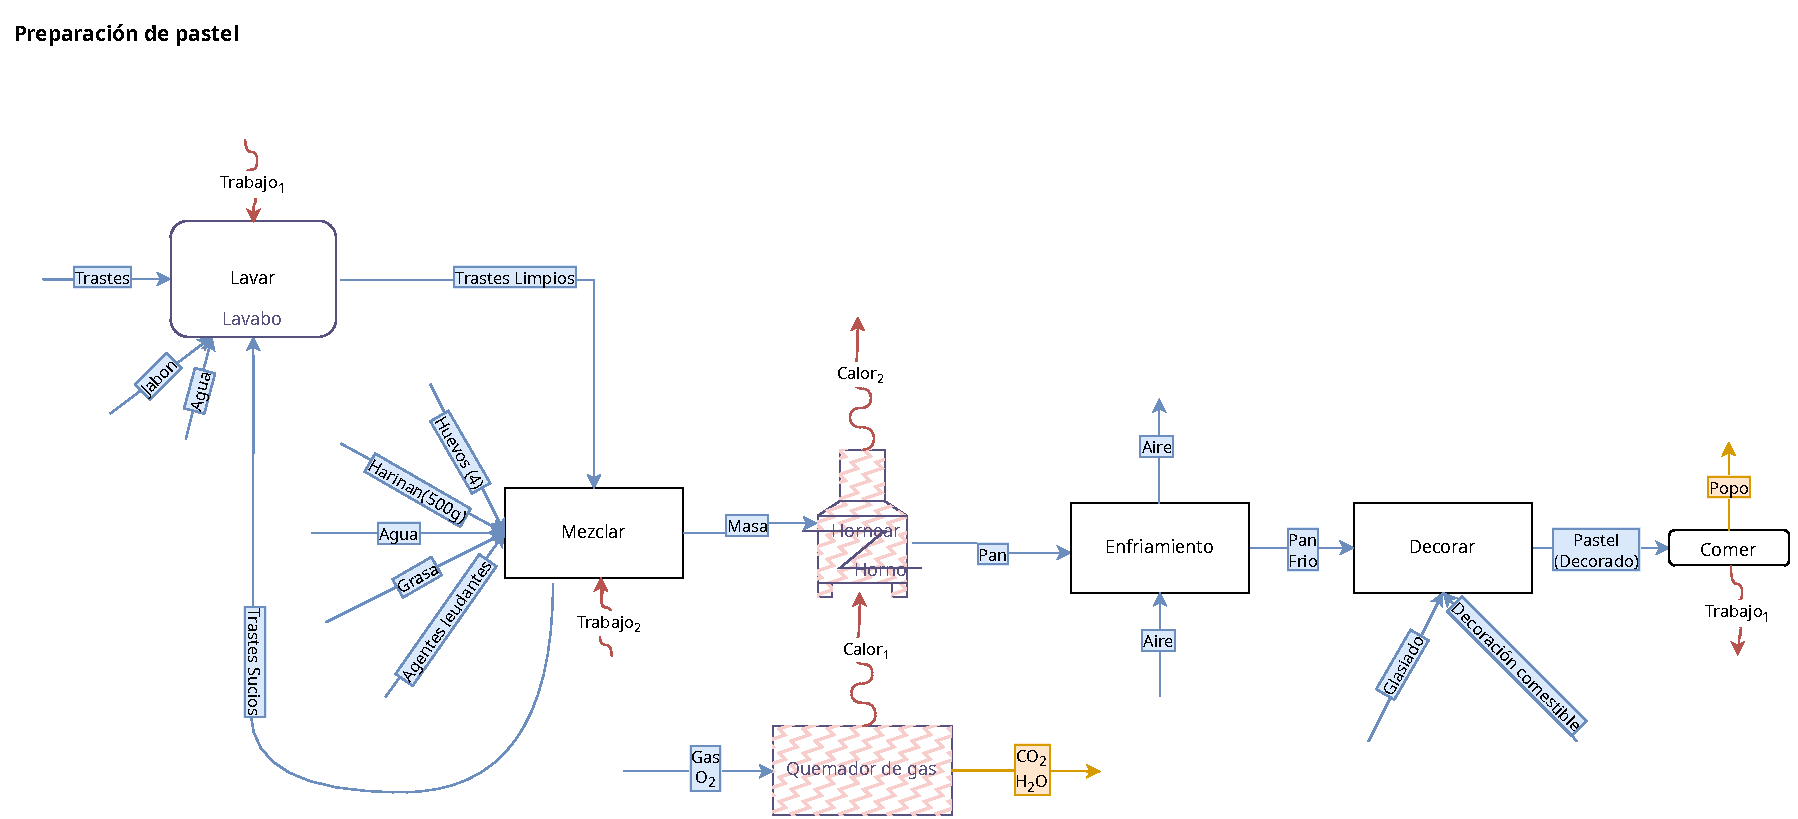
\includegraphics[width=\textwidth]{Diagramas/diagrama/Diagrama_pastel.pdf}
\end{center}

\begin{notaimportante}
\textbf{Sobre el nivel de detalle de este DFP.} En la sección anterior
se indicó que el DFP debe mantenerse lo más limpio posible: sin
anotaciones encima de las corrientes, solo números, máquinas y flujos
de energía. En este ejemplo se usó más texto del habitual porque el
objetivo de la actividad era exclusivamente construir el diagrama. Al
no haber ejercicio numérico que resolver, no hay tablas de corrientes
donde poner los datos, y la información se anotó directamente sobre el
diagrama. En ejercicios posteriores con cálculos, se sigue el criterio
estricto: corrientes numeradas, datos en tablas aparte.
\end{notaimportante}

\phantomsection
\addcontentsline{toc}{subsubsection}{Clase 3 -- 24/08/2026: De texto a DFP y tabla de corrientes}
\subsubsection*{\textcolor{blueunam}{Clase 3 -- 24/08/2026: De texto a DFP y tabla de corrientes}}

\textbf{Tablas de corrientes.} La información de cada corriente
(flujo, composición, temperatura, presión) no se anota en el DFP. Se
organiza en una \textbf{tabla de corrientes} aparte. La convención
del curso es:

\begin{itemize}
    \item Cada \textbf{corriente} ocupa un \textbf{renglón}. La
    primera columna lleva el número de corriente encerrado en un
    círculo.
    \item Cada \textbf{variable} ocupa una \textbf{columna}, con su
    unidad en el encabezado.
    \item Las conversiones se hacen antes de armar la tabla, no
    dentro de ella.
\end{itemize}

Una tabla típica tiene esta estructura:

\begin{center}
\renewcommand{\arraystretch}{1.6}
\begin{tabularx}{\textwidth}{|c|X|X|X|X|}
\hline
\textbf{Corriente} & \textbf{T ($^\circ$C)} & \textbf{T (K)} &
\textbf{T ($^\circ$F)} & \textbf{T ($^\circ$R)} \\
\hline
\corriente{1} & & & & \\
\hline
\corriente{2} & & & & \\
\hline
\corriente{3} & & & & \\
\hline
\end{tabularx}
\end{center}

\begin{notaimportante}
No todas las columnas se usan siempre. Si el problema no tiene datos
de presión, no se pone la columna. Si no hay composición porque el
fluido es puro, se puede omitir o indicar ``puro''. La tabla se adapta
al ejercicio, no al revés.
\end{notaimportante}

\textbf{Flujo de trabajo.} Todo ejercicio de proceso sigue el mismo
orden:

\begin{enumerate}
    \item Leer el enunciado y dibujar el DFP.
    \item Convertir los datos a las \textbf{mismas unidades}, si es
    necesario. La conversión se hace al lado, en el margen, o en el
    espacio de trabajo, no como una tabla aparte.
    \item Armar la tabla con los datos ya convertidos.
    \item Plantear las ecuaciones: de balance, de total, y las
    relaciones adicionales que dé el enunciado.
    \item Resolver y verificar.
\end{enumerate}

El paso 2 solo aplica si los datos vienen en unidades distintas. Si
ya están en la misma unidad, se pasa directo del paso 1 al 3. La
tabla es una sola: la definitiva.

\begin{notaimportante}
\textbf{Sobre las corrientes de servicio.} Los equipos de intercambio
térmico (intercambiadores, condensadores, rehervidores, calentadores,
enfriadores) tienen, además de las corrientes de proceso, una o dos
corrientes de \textbf{servicio}: agua de enfriamiento, vapor, aceite
térmico, refrigerante. Esas corrientes existen físicamente y son
parte del equipo, pero en los ejercicios de balance \textbf{no se
analizan}: solo se estudian las corrientes de proceso.

En el DFP se dibujan por formalismo, para que el diagrama sea
completo y coherente con el equipo. Pero no se incluyen en la tabla
de corrientes ni en los cálculos, a menos que el enunciado lo pida
explícitamente. Lo mismo aplica a las pérdidas de calor al ambiente
en tuberías o equipos sin aislamiento.

Esta simplificación es una convención didáctica. En un problema real
de diseño, todas las corrientes se analizan y se dimensionan. En este
curso, se trabaja solo con las corrientes de proceso.
\end{notaimportante}

% ══════════════════════════════════════════════════════════════
%  EJERCICIOS DE CONVERSIÓN APLICADOS A TABLAS
% ══════════════════════════════════════════════════════════════

\textbf{Ejercicios de conversión aplicados a tablas.}

Los siguientes ejercicios entrenan el flujo de trabajo completo:
leer el enunciado, construir el DFP, organizar los datos en la tabla,
convertir unidades y llenar la tabla final. No se piden balances.

\begin{exercise}{9}{}
En un tanque se mezclan dos corrientes de agua: una a $70\,^\circ$C y
otra a $15\,^\circ$C. Si el balance final da como resultado
$40\,\mathrm{L}$ de agua a $37\,^\circ$C, ¿qué volumen se empleó de
agua caliente y qué volumen de agua fría? Considera que la densidad
del agua es $1\,\mathrm{kg/L}$ y que no hay pérdidas de calor.

Llena la tabla de corrientes con cada temperatura expresada en las
cuatro escalas ($^\circ$C, K, $^\circ$F, $^\circ$R).

Solución:

\textit{Paso 1. DFP del proceso.}

\begin{center}
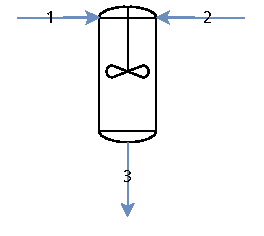
\includegraphics[width=0.55\textwidth]{Diagramas/diagrama/Diagrama_agua_caliente.pdf}
\end{center}

\textit{Paso 2. Tabla de corrientes.}

\begin{center}
\renewcommand{\arraystretch}{1.6}
\begin{tabularx}{\textwidth}{|c|X|X|X|X|}
\hline
\textbf{Corriente} & \textbf{T ($^\circ$C)} & \textbf{T (K)} &
\textbf{T ($^\circ$F)} & \textbf{T ($^\circ$R)} \\
\hline
\corriente{1} & $70$ & $T_1$ & $T_1$ & $T_1$ \\
\hline
\corriente{2} & $15$ & $T_2$ & $T_2$ & $T_2$ \\
\hline
\corriente{3} & $37$ & $T_3$ & $T_3$ & $T_3$ \\
\hline
\end{tabularx}
\end{center}

\textit{Paso 3. Conversión de unidades.}

Corriente 1:
\begin{align*}
T_1(\mathrm{K}) &= 70 + 273.15 = 343.15\,\mathrm{K} \\[4pt]
T_1(^\circ\mathrm{F}) &= 1.8(70) + 32 = 158\,^\circ\mathrm{F} \\[4pt]
T_1(^\circ\mathrm{R}) &= 158 + 459.67 = 617.67\,^\circ\mathrm{R}
\end{align*}

Corriente 2:
\begin{align*}
T_2(\mathrm{K}) &= 15 + 273.15 = 288.15\,\mathrm{K} \\[4pt]
T_2(^\circ\mathrm{F}) &= 1.8(15) + 32 = 59\,^\circ\mathrm{F} \\[4pt]
T_2(^\circ\mathrm{R}) &= 59 + 459.67 = 518.67\,^\circ\mathrm{R}
\end{align*}

Corriente 3:
\begin{align*}
T_3(\mathrm{K}) &= 37 + 273.15 = 310.15\,\mathrm{K} \\[4pt]
T_3(^\circ\mathrm{F}) &= 1.8(37) + 32 = 98.6\,^\circ\mathrm{F} \\[4pt]
T_3(^\circ\mathrm{R}) &= 98.6 + 459.67 = 558.27\,^\circ\mathrm{R}
\end{align*}

\textit{Paso 4. Tabla final.}

\begin{center}
\renewcommand{\arraystretch}{1.6}
\begin{tabularx}{\textwidth}{|c|X|X|X|X|}
\hline
\textbf{Corriente} & \textbf{T ($^\circ$C)} & \textbf{T (K)} &
\textbf{T ($^\circ$F)} & \textbf{T ($^\circ$R)} \\
\hline
\corriente{1} & 70 & 343.15 & 158 & 617.67 \\
\hline
\corriente{2} & 15 & 288.15 & 59 & 518.67 \\
\hline
\corriente{3} & 37 & 310.15 & 98.6 & 558.27 \\
\hline
\end{tabularx}
\end{center}
\end{exercise}

\begin{exercise}{10}{}
Una corriente de agua de enfriamiento entra a un intercambiador de
calor a $75\,^\circ$F. Durante su paso por el equipo, el agua
experimenta un incremento de temperatura de $15\,^\circ$C. Determina
las temperaturas de entrada y salida en las cuatro escalas
($^\circ$C, K, $^\circ$F, $^\circ$R) y organiza la información en una
tabla de corrientes.

Solución:

\textit{Paso 1. DFP del proceso.}

\begin{center}
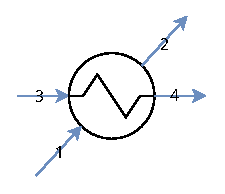
\includegraphics[width=0.55\textwidth]{Diagramas/diagrama/Diagrama_intercambiador.pdf}
\end{center}

\textit{Paso 2. Conversión de unidades.}

Entrada:
\begin{align*}
T_1(^\circ\mathrm{C}) &= \frac{75 - 32}{1.8} = 23.89\,^\circ\mathrm{C} \\[4pt]
T_1(\mathrm{K}) &= 23.89 + 273.15 = 297.04\,\mathrm{K} \\[4pt]
T_1(^\circ\mathrm{R}) &= 75 + 459.67 = 534.67\,^\circ\mathrm{R}
\end{align*}

Salida: el incremento es de $15\,^\circ$C, que equivale a $15\,\mathrm{K}$:
\begin{align*}
T_2(^\circ\mathrm{C}) &= T_1(^\circ\mathrm{C}) + 15 = 38.89\,^\circ\mathrm{C} \\[4pt]
T_2(\mathrm{K}) &= T_1(\mathrm{K}) + 15 = 312.04\,\mathrm{K} \\[4pt]
T_2(^\circ\mathrm{F}) &= 1.8(38.89) + 32 = 102.0\,^\circ\mathrm{F} \\[4pt]
T_2(^\circ\mathrm{R}) &= 102.0 + 459.67 = 561.67\,^\circ\mathrm{R}
\end{align*}

\textit{Paso 3. Tabla de corrientes.}

\begin{center}
\renewcommand{\arraystretch}{1.6}
\begin{tabularx}{\textwidth}{|c|X|X|X|X|}
\hline
\textbf{Corriente} & \textbf{T ($^\circ$C)} & \textbf{T (K)} &
\textbf{T ($^\circ$F)} & \textbf{T ($^\circ$R)} \\
\hline
\corriente{1} & 23.89 & 297.04 & 75 & 534.67 \\
\hline
\corriente{2} & 38.89 & 312.04 & 102.0 & 561.67 \\
\hline
\end{tabularx}
\end{center}

{\small\itshape
\textbf{Verificación:} $T_2(^\circ\mathrm{C}) - T_1(^\circ\mathrm{C}) =
38.89 - 23.89 = 15\,^\circ$C, y en escala Fahrenheit
$T_2(^\circ\mathrm{F}) - T_1(^\circ\mathrm{F}) = 102.0 - 75 = 27\,^\circ$F,
que equivale a $27 \times 5/9 = 15\,^\circ$C. Correcto.
}
\end{exercise}

\begin{exercise}{11}{}
Vapor sobrecalentado a $420\,^\circ$C viaja por una tubería sin
suficiente aislamiento térmico. Debido a las pérdidas ambientales
hacia el entorno, el vapor sufre una caída de temperatura de
$80\,\mathrm{K}$. Determina las temperaturas de entrada y salida en
las cuatro escalas ($^\circ$C, K, $^\circ$F, $^\circ$R) y organiza la
información en una tabla de corrientes.

Solución:

\textit{Paso 1. DFP del proceso.}

\begin{center}
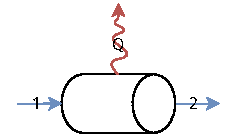
\includegraphics[width=0.55\textwidth]{Diagramas/diagrama/Diagrama_tuberia.pdf}
\end{center}

\textit{Paso 2. Conversión de unidades.}

Entrada:
\begin{align*}
T_1(\mathrm{K}) &= 420 + 273.15 = 693.15\,\mathrm{K} \\[4pt]
T_1(^\circ\mathrm{F}) &= 1.8(420) + 32 = 788\,^\circ\mathrm{F} \\[4pt]
T_1(^\circ\mathrm{R}) &= 788 + 459.67 = 1247.67\,^\circ\mathrm{R}
\end{align*}

Salida: la caída es de $80\,\mathrm{K}$, que equivale a $80\,^\circ$C:
\begin{align*}
T_2(^\circ\mathrm{C}) &= 420 - 80 = 340\,^\circ\mathrm{C} \\[4pt]
T_2(\mathrm{K}) &= 693.15 - 80 = 613.15\,\mathrm{K} \\[4pt]
T_2(^\circ\mathrm{F}) &= 1.8(340) + 32 = 644\,^\circ\mathrm{F} \\[4pt]
T_2(^\circ\mathrm{R}) &= 644 + 459.67 = 1103.67\,^\circ\mathrm{R}
\end{align*}

\textit{Paso 3. Tabla de corrientes.}

\begin{center}
\renewcommand{\arraystretch}{1.6}
\begin{tabularx}{\textwidth}{|c|X|X|X|X|}
\hline
\textbf{Corriente} & \textbf{T ($^\circ$C)} & \textbf{T (K)} &
\textbf{T ($^\circ$F)} & \textbf{T ($^\circ$R)} \\
\hline
\corriente{1} & 420 & 693.15 & 788 & 1247.67 \\
\hline
\corriente{2} & 340 & 613.15 & 644 & 1103.67 \\
\hline
\end{tabularx}
\end{center}

{\small\itshape
\textbf{Verificación:} $T_1(^\circ\mathrm{C}) - T_2(^\circ\mathrm{C}) =
420 - 340 = 80\,^\circ$C, y en escala Fahrenheit
$T_1(^\circ\mathrm{F}) - T_2(^\circ\mathrm{F}) = 788 - 644 = 144\,^\circ$F,
que equivale a $144 \times 5/9 = 80\,^\circ$C. Correcto.
}
\end{exercise}

\begin{exercise}{12}{}
El agua de un circuito de enfriamiento entra a un condensador a
$22\,^\circ$C y se calienta hasta $564\,\mathrm{R}$. Determina las
temperaturas de entrada y salida en las cuatro escalas
($^\circ$C, K, $^\circ$F, $^\circ$R) y organiza la información en una
tabla de corrientes.

Solución:

\textit{Paso 1. DFP del proceso.}

\begin{center}
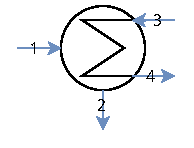
\includegraphics[width=0.55\textwidth]{Diagramas/diagrama/Diagrama_condensador.pdf}
\end{center}

\textit{Paso 2. Conversión de unidades.}

Entrada ($22\,^\circ$C):
\begin{align*}
T_1(\mathrm{K}) &= 22 + 273.15 = 295.15\,\mathrm{K} \\[4pt]
T_1(^\circ\mathrm{F}) &= 1.8(22) + 32 = 71.6\,^\circ\mathrm{F} \\[4pt]
T_1(^\circ\mathrm{R}) &= 71.6 + 459.67 = 531.27\,^\circ\mathrm{R}
\end{align*}

Salida ($564\,\mathrm{R}$):
\begin{align*}
T_2(^\circ\mathrm{F}) &= 564 - 459.67 = 104.33\,^\circ\mathrm{F} \\[4pt]
T_2(^\circ\mathrm{C}) &= \frac{104.33 - 32}{1.8} = 40.18\,^\circ\mathrm{C} \\[4pt]
T_2(\mathrm{K}) &= 40.18 + 273.15 = 313.33\,\mathrm{K}
\end{align*}

\textit{Paso 3. Tabla de corrientes.}

\begin{center}
\renewcommand{\arraystretch}{1.6}
\begin{tabularx}{\textwidth}{|c|X|X|X|X|}
\hline
\textbf{Corriente} & \textbf{T ($^\circ$C)} & \textbf{T (K)} &
\textbf{T ($^\circ$F)} & \textbf{T ($^\circ$R)} \\
\hline
\corriente{1} & 22 & 295.15 & 71.6 & 531.27 \\
\hline
\corriente{2} & 40.18 & 313.33 & 104.33 & 564 \\
\hline
\end{tabularx}
\end{center}

{\small\itshape
\textbf{Verificación:} $T_2(^\circ\mathrm{C}) - T_1(^\circ\mathrm{C}) =
40.18 - 22 = 18.18\,^\circ$C. En escala Kelvin,
$313.33 - 295.15 = 18.18\,\mathrm{K}$. En escala Fahrenheit,
$104.33 - 71.6 = 32.73\,^\circ$F, que equivale a
$32.73 \times 5/9 = 18.18\,^\circ$C. Correcto.
}
\end{exercise}

\begin{notaimportante}
Los ejercicios de esta sección no piden balances. El objetivo es
practicar el flujo de trabajo: leer el texto, construir el DFP,
organizar los datos en la tabla, convertir unidades y llenar la tabla
final. Los balances de materia y energía se verán a partir de la
siguiente clase.
\end{notaimportante}

% ══════════════════════════════════════════════════════════════
%  CLASE 4
% ══════════════════════════════════════════════════════════════

\phantomsection
\addcontentsline{toc}{subsubsection}{Clase 4 -- 30/08/2026: Flujo y régimen permanente}
\subsubsection*{\textcolor{blueunam}{Clase 4 -- 30/08/2026: Flujo y régimen permanente}}

\textbf{Flujo:} cantidad de masa, mol o volumen que entra o sale de un
sistema. Puede expresarse en unidades de cantidad total o de cantidad
por tiempo.

De las tres, el flujo en \textbf{masa} o en \textbf{mol} es el
preferido. El flujo volumétrico es menos común porque el volumen de
una sustancia cambia con la temperatura y la presión: si se calienta
se expande, si se enfría se contrae, aunque su masa y su cantidad de
sustancia permanezcan iguales. Masa y mol, en cambio, no cambian con
esas condiciones. Si en algún momento se necesita el volumen, se
calcula a partir de la densidad.

\textbf{Tipos de flujo.}

\begin{itemize}
    \item \textbf{Flujo total:} cantidad de masa o mol que entra o
    sale del sistema en todo el proceso, sin referencia al tiempo. Se
    usa en procesos por lotes, donde importa cuánto se procesó al
    final y no a qué velocidad.
    \item \textbf{Flujo por tiempo:} cantidad de masa o mol que entra
    o sale del sistema por unidad de tiempo. Se usa en procesos
    continuos y es el más común en BME.
\end{itemize}

\begin{center}
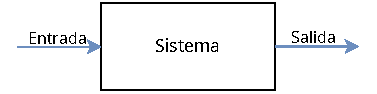
\includegraphics[width=0.55\textwidth]{Diagramas/diagrama/Diagrama_Sistema.pdf}
\end{center}

El diagrama muestra la idea básica de todo sistema: algo entra, algo
sale, y dentro ocurre un proceso que puede o no transformar lo que
entró. Lo que está dentro del rectángulo es el \textbf{sistema}; las
flechas que apuntan hacia él son las \textbf{entradas}, y las que
salen, las \textbf{salidas}. Esta imagen es la base de todo balance:
contar lo que entra, contar lo que sale, y comparar.

\textbf{Ecuación general de balance.} Para cualquier sistema, sin
importar su naturaleza, se cumple que: \\
$\text{Final} - \text{Inicial} = \text{Entrada} - \text{Salida} + \text{Generado} - \text{Consumido}$,
donde \textit{Final $-$ Inicial} es la \textbf{acumulación}.

\begin{itemize}
    \item \textbf{Final $-$ Inicial:} acumulación. Lo que cambió
    dentro del sistema entre el inicio y el final del proceso.
    \item \textbf{Entrada $-$ Salida:} flujo neto. Lo que entró menos
    lo que salió por las fronteras del sistema.
    \item \textbf{Generado:} lo que aparece dentro del sistema por
    reacción química u otra transformación.
    \item \textbf{Consumido:} lo que desaparece dentro del sistema
    por reacción química u otra transformación.
\end{itemize}

\begin{notadidactica}
\textbf{El ejemplo de los aviones de papel.} Imagina que tienes una
colección de aviones de papel. Al inicio del día tienes cierta
cantidad. Durante el día fabricas más, regalas algunos, compras otros,
y algunos se rompen. Al final del día, ¿cuántos tienes?

La cuenta es intuitiva: los aviones finales son iguales a los que
tenías al inicio, más los que entraron (fabricaste o compraste), menos
los que salieron (regalaste o vendiste), más los que se generaron
dentro del sistema (los que fabricaste con material que ya tenías),
menos los que se consumieron (los que se rompieron o destruyeron).

Esa misma lógica aplica a cualquier sistema, desde un tanque hasta un
reactor. La ecuación general no es más que esa cuenta, escrita de
forma que sirva para todo.
\end{notadidactica}

\textbf{Notación de flujo.} A partir de aquí, a cualquier tipo de
flujo se le llamará simplemente \textbf{flujo}, y el tipo se
identifica por sus unidades. La notación general es una letra con un
punto arriba: $\dot{x}$, donde el punto indica que es una cantidad por
unidad de tiempo. Los casos específicos más usados son:

\begin{itemize}
    \item Flujo másico: $\dot{m}$, en $\mathrm{kg/s}$,
    $\mathrm{kg/h}$, $\mathrm{lb/min}$, etc.
    \item Flujo molar: $\dot{n}$, en $\mathrm{mol/s}$,
    $\mathrm{kmol/h}$, $\mathrm{lbmol/min}$, etc.
    \item Flujo volumétrico: $\dot{V}$, en $\mathrm{m^3/s}$,
    $\mathrm{L/min}$, $\mathrm{ft^3/h}$, etc.
\end{itemize}

\textbf{Forma diferencial de la ecuación de balance.} La ecuación
general puede escribirse en términos de flujos, derivando respecto al
tiempo:

\[
\frac{dx}{dt} = \dot{\text{Entrada}} - \dot{\text{Salida}}
+ \dot{\text{Generación}} - \dot{\text{Consumo}}
\]

donde $x$ es la cantidad acumulada y puede ser masa ($m$), cantidad
de sustancia ($n$) o volumen ($V$), según lo que se esté analizando.
El término $\frac{dx}{dt}$ es la acumulación.

\textbf{Diferencia con la ecuación general.} En la ecuación general
los términos son \textbf{cantidades} (masa, mol o volumen totales,
sin referencia al tiempo). En la forma diferencial, todos los
términos son \textbf{flujos}: llevan punto arriba y están en unidades
de cantidad por tiempo, $[U/t]$. Es decir, la forma diferencial no
solo agrega la derivada: cambia la naturaleza de cada término, de
cantidad a flujo.

\textbf{Régimen permanente.} En este curso se trabajará mucho con
esta condición. Se refiere a cuando la acumulación es cero:
$\frac{dx}{dt} = 0$. La ecuación se reduce a:

\[
0 = \dot{\text{Entrada}} - \dot{\text{Salida}}
+ \dot{\text{Generación}} - \dot{\text{Consumo}}
\]

o, reordenando:

\[
\dot{\text{Entrada}} + \dot{\text{Generación}}
= \dot{\text{Salida}} + \dot{\text{Consumo}}
\]

\begin{notaimportante}
No siempre se genera ni se consume. De hecho, al principio del curso
será raro ver que estos términos sean distintos de cero, porque la
mayoría de los ejercicios no involucran reacción química. Pero puede
llegar a pasar, así que en los ejercicios siempre se escribirá la
ecuación completa y se simplificará según el tipo de sistema.
\end{notaimportante}

\textbf{Promedios.} En BME es común trabajar con mezclas, y para hacer
conversiones entre masa y mol se necesita un valor promedio de las
propiedades. Los dos promedios más usados son la masa molar promedio
y la composición promedio.

\textbf{Masa molar promedio ($\overline{MM}$).} Es la masa molar de
una mezcla, calculada como el promedio ponderado por la fracción mol
de cada componente:

\[
\overline{MM} = \sum_{j=1}^{k} \chi_j \, MM_j
\]

donde $\chi_j$ es la fracción mol del componente $j$, $MM_j$ su masa
molar, y $k$ el número de componentes de la mezcla. Se usa para
convertir entre masa y mol de una mezcla cuando no se conoce la
composición individual de cada corriente.

\textbf{Composición promedio.} Para una corriente que es mezcla de
varias, la composición se expresa como fracción (o porcentaje) de cada
componente. Hay dos formas comunes:

\begin{itemize}
    \item \textbf{Fracción mol ($\chi_i$):} mol de $i$ entre mol total.
    Se usa en cálculos con gases y en balances molares.
    \[
    \chi_i = \frac{n_i}{n_{\text{total}}}, \qquad \sum_{j=1}^{k} \chi_j = 1
    \]
    \item \textbf{Fracción masa ($w_i$):} masa de $i$ entre masa
    total. Se usa en cálculos con líquidos y sólidos, y en balances
    másicos.
    \[
    w_i = \frac{m_i}{m_{\text{total}}}, \qquad \sum_{j=1}^{k} w_j = 1
    \]
\end{itemize}

\textbf{Conversión entre fracción mol y fracción masa.} Sea $k$ el
número de componentes de la mezcla:

\[
w_i = \frac{\chi_i \, MM_i}{\displaystyle\sum_{j=1}^{k} \chi_j \, MM_j}
\qquad \Longleftrightarrow \qquad
\chi_i = \frac{w_i}{MM_i \cdot \displaystyle\sum_{j=1}^{k} \left( w_j / MM_j \right)}
\]

El denominador de la primera expresión es la masa molar promedio de
la mezcla. El denominador de la segunda es $MM_i$ multiplicado por el
total de moles por unidad de masa de mezcla.

\begin{notafija}
\textbf{Sobre los índices $i$ y $j$.} $i$ identifica el componente
que se está calculando y se mantiene fijo durante todo el cálculo.
$j$ toma cada uno de los componentes dentro de la sumatoria, uno por
uno. Se usan letras distintas para evitar ambigüedad.

La sumatoria incluye al mismo componente $i$ que aparece en el
numerador. Por ejemplo, si se calcula la fracción masa del oxígeno en
aire, el término del oxígeno aparece tanto arriba como dentro de la
suma del denominador, porque el oxígeno es parte de la mezcla y a la
vez es lo que se está midiendo contra el total.
\end{notafija}

\textbf{Ejemplo.} El aire seco tiene una composición aproximada de
$21\%$ mol de \ce{O2} y $79\%$ mol de \ce{N2}. Su masa molar
promedio es:

\[
\overline{MM} = (0.21)(32.00) + (0.79)(28.01)
= 6.72 + 22.13 = 28.85\,\frac{\mathrm{g}}{\mathrm{mol}}
\]

El valor que se usa normalmente ($28.97\,\mathrm{g/mol}$) incluye
otros componentes minoritarios como \ce{Ar} y \ce{CO2}, pero el
cálculo es el mismo.

Con esa masa molar promedio se puede convertir entre masa y mol de
aire. También se puede calcular la fracción masa del \ce{O2}:

\[
w_{\ce{O2}} = \frac{\chi_{\ce{O2}} \, MM_{\ce{O2}}}{\overline{MM}}
= \frac{(0.21)(32.00)}{28.85} = 0.233
\]

Es decir, aunque el \ce{O2} es el $21\%$ mol del aire, es el $23.3\%$
masa, porque sus moléculas son más pesadas que las de \ce{N2}.

Este tipo de promedio es el que se usó en el ejercicio del ventilador
para convertir entre masa y mol de aire.

\textbf{Ejercicios de conversión de flujo.}

Estos ejercicios no requieren DFP: no hay un sistema con corrientes,
solo una cantidad de flujo que se expresa en distintas unidades. El
objetivo es manejar con soltura las conversiones entre masa, mol y
volumen, y entre unidades de tiempo.

\begin{exercise}{13}{}
Un flujo másico de $250\,\mathrm{kg/h}$ de agua circula por una
tubería. Expresa este flujo en $\mathrm{mol/s}$ y en
$\mathrm{lb/min}$.

Solución:

\textit{Paso 1. Datos y unidades objetivo.}

\[
\dot{m} = 250\,\frac{\mathrm{kg}}{\mathrm{h}}
\quad \longrightarrow \quad
\dot{n} = ?\,\frac{\mathrm{mol}}{\mathrm{s}}
\qquad
\dot{m} = ?\,\frac{\mathrm{lb}}{\mathrm{min}}
\]

\textit{Paso 2. Conversión a mol/s.}

Primero pasamos de masa a mol usando la masa molar del agua
($MM_{\ce{H2O}} = 18.016\,\mathrm{g/mol}$):
\[
\dot{n} = 250\,\frac{\mathrm{kg}}{\mathrm{h}}
\times \frac{1000\,\mathrm{g}}{1\,\mathrm{kg}}
\times \frac{1\,\mathrm{mol}}{18.016\,\mathrm{g}}
= 13876\,\frac{\mathrm{mol}}{\mathrm{h}}
\]
Luego convertimos horas a segundos:
\[
\dot{n} = 13876\,\frac{\mathrm{mol}}{\mathrm{h}}
\times \frac{1\,\mathrm{h}}{3600\,\mathrm{s}}
= 3.854\,\frac{\mathrm{mol}}{\mathrm{s}}
\]

\textit{Paso 3. Conversión a lb/min.}

\[
\dot{m} = 250\,\frac{\mathrm{kg}}{\mathrm{h}}
\times \frac{2.205\,\mathrm{lb}}{1\,\mathrm{kg}}
\times \frac{1\,\mathrm{h}}{60\,\mathrm{min}}
= 9.188\,\frac{\mathrm{lb}}{\mathrm{min}}
\]

\textit{Paso 4. Tabla de resultados.}

\begin{center}
\renewcommand{\arraystretch}{1.6}
\begin{tabularx}{\textwidth}{|c|X|X|X|}
\hline
\textbf{Variable} & \textbf{Valor original} &
\textbf{En mol/s} & \textbf{En lb/min} \\
\hline
Flujo de agua & $250\,\mathrm{kg/h}$ & 3.854 & 9.188 \\
\hline
\end{tabularx}
\end{center}

\end{exercise}

\begin{exercise}{14}{}
Un ventilador introduce aire a un departamento con un caudal de
$60\,\mathrm{SCFM}$ (pies cúbicos estándar por minuto). Determina la
equivalencia de este caudal en:

\begin{enumerate}[a)]
    \item moles por hora.
    \item kilogramos por día.
    \item metros cúbicos por minuto, considerando que en el
    departamento el aire está a $25\,^\circ$C y $585\,\mathrm{Torr}$.
\end{enumerate}

Asume que el aire se comporta como gas ideal, con una masa molar
promedio de $28.97\,\mathrm{g/mol}$. Considera condiciones estándar de
$0\,^\circ$C y $1\,\mathrm{atm}$.

Solución:

\textit{Paso 1. Datos.}
\begin{align*}
\dot{V} &= 60\,\frac{\mathrm{ft^3}}{\mathrm{min}} \;\text{(SCFM)} \\[4pt]
MM_{\text{aire}} &= 28.97\,\frac{\mathrm{g}}{\mathrm{mol}} \\[4pt]
\text{Estándar:} &\quad 0\,^\circ\mathrm{C},\; 1\,\mathrm{atm} \\[4pt]
\text{Departamento:} &\quad 25\,^\circ\mathrm{C},\; 585\,\mathrm{Torr}
\end{align*}

\textit{Paso 2. Volumen molar en condiciones estándar.}

En condiciones estándar ($0\,^\circ$C, $1\,\mathrm{atm}$), un mol de
gas ideal ocupa:
\[
V_m = \frac{RT}{P}
= \frac{(0.08206\,\mathrm{L\cdot atm/(mol\cdot K)})(273.15\,\mathrm{K})}{1\,\mathrm{atm}}
= 22.414\,\frac{\mathrm{L}}{\mathrm{mol}}
\]

\textit{Paso 3. Conversión a mol/h.}

Primero llevamos el caudal a litros por minuto para usar directamente
el volumen molar:
\[
\dot{V} = 60\,\frac{\mathrm{ft^3}}{\mathrm{min}}
\times \frac{28.317\,\mathrm{L}}{1\,\mathrm{ft^3}}
= 1699\,\frac{\mathrm{L}}{\mathrm{min}}
\]

Ahora aplicamos el volumen molar estándar:
\[
\dot{n} = 1699\,\frac{\mathrm{L}}{\mathrm{min}}
\times \frac{1\,\mathrm{mol}}{22.414\,\mathrm{L}}
\times \frac{60\,\mathrm{min}}{1\,\mathrm{h}}
= 4548\,\frac{\mathrm{mol}}{\mathrm{h}}
\]

\textit{Paso 4. Conversión a kg/día.}

\[
\dot{m} = 4548\,\frac{\mathrm{mol}}{\mathrm{h}}
\times \frac{28.97\,\mathrm{g}}{1\,\mathrm{mol}}
\times \frac{1\,\mathrm{kg}}{1000\,\mathrm{g}}
\times \frac{24\,\mathrm{h}}{1\,\mathrm{d\acute{i}a}}
= 3162\,\frac{\mathrm{kg}}{\mathrm{d\acute{i}a}}
\]

\textit{Paso 5. Conversión a m$^3$/min a $25\,^\circ$C y $585\,\mathrm{Torr}$.}

El caudal molar no cambia con las condiciones: el mismo número de
moles entra al departamento. Lo que cambia es el volumen que ocupan.
Para verlo con números, calculamos el caudal volumétrico en las dos
condiciones usando $P\dot{V} = \dot{n}RT$ con el mismo $\dot{n}$.

\textit{En condiciones estándar} ($0\,^\circ$C, $1\,\mathrm{atm}$):
\[
\dot{V}_1 = \frac{\dot{n}RT_1}{P_1}
= \frac{(4548)(0.08206)(273.15)}{1}
= 101{,}930\,\frac{\mathrm{L}}{\mathrm{h}}
\]

\textit{En el departamento} ($25\,^\circ$C, $585\,\mathrm{Torr}$):
\[
\dot{V}_2 = \frac{\dot{n}RT_2}{P_2}
= \frac{(4548)(0.08206)(298.15)}{0.7697}
= 144{,}560\,\frac{\mathrm{L}}{\mathrm{h}}
\]

\begin{center}
\renewcommand{\arraystretch}{1.6}
\begin{tabularx}{\textwidth}{|X|X|X|}
\hline
\textbf{Condición} & \textbf{Caudal molar (mol/h)} &
\textbf{Caudal volumétrico (L/h)} \\
\hline
Estándar ($0\,^\circ$C, $1\,\mathrm{atm}$) & 4548 & 101{,}930 \\
\hline
Departamento ($25\,^\circ$C, $585\,\mathrm{Torr}$) & 4548 & 144{,}560 \\
\hline
\end{tabularx}
\end{center}

La diferencia entre ambos caudales volumétricos se explica por la
razón entre las condiciones:
\[
\frac{\dot{V}_2}{\dot{V}_1}
= \frac{T_2}{T_1} \cdot \frac{P_1}{P_2}
= \frac{298.15}{273.15} \cdot \frac{760}{585}
= 1.0915 \times 1.2991 = 1.418
\]
El volumen crece un $41.8\%$ porque la temperatura sube (factor
$1.0915$) y la presión baja (factor $1.2991$). Los moles son los
mismos; solo ocupan más espacio.

Finalmente, convertimos $\dot{V}_2$ a metros cúbicos por minuto:
\[
\dot{V}_2 = 144{,}560\,\frac{\mathrm{L}}{\mathrm{h}}
\times \frac{1\,\mathrm{m^3}}{1000\,\mathrm{L}}
\times \frac{1\,\mathrm{h}}{60\,\mathrm{min}}
= 2.409\,\frac{\mathrm{m^3}}{\mathrm{min}}
\]

\textit{Paso 6. Resultados.}
\begin{align*}
\text{a)}\quad \dot{n} &= 4548\,\frac{\mathrm{mol}}{\mathrm{h}} \\[4pt]
\text{b)}\quad \dot{m} &= 3162\,\frac{\mathrm{kg}}{\mathrm{d\acute{i}a}} \\[4pt]
\text{c)}\quad \dot{V}_2 &= 2.409\,\frac{\mathrm{m^3}}{\mathrm{min}}
\;\text{(a $25\,^\circ$C, $585\,\mathrm{Torr}$)}
\end{align*}
\end{exercise}

\textbf{Por qué se prefiere masa o mol sobre volumen.} Este ejercicio
deja ver el problema de medir flujos en volumen. Para pasar de
$\mathrm{ft^3/min}$ a $\mathrm{mol/h}$ solo fue necesario saber que se
trata de aire, su masa molar promedio, y las conversiones entre
unidades. Para pasar a $\mathrm{kg/d\acute{i}a}$, lo mismo. En cambio,
para expresar el caudal en volumen a las condiciones del departamento
fue necesario conocer \textbf{todas} las condiciones: temperatura y
presión. Y aun así, el resultado es una aproximación que asume
comportamiento de gas ideal.

Con masa o mol, la cantidad no cambia con las condiciones. Con volumen,
sí. Por eso en BME se trabaja preferentemente en masa o mol: son
cantidades que no dependen de la temperatura ni la presión, y que
además se conservan en los balances. El volumen, en cambio, no se
conserva.

% ══════════════════════════════════════════════════════════════
%  ECUACIONES DE BALANCE DE MATERIA
% ══════════════════════════════════════════════════════════════

\textbf{Ecuaciones de balance de materia.} La ecuación general de
balance es una sola:

\[
\text{Acu} = \text{Ent} - \text{Sal} + \text{Rx}
\]

donde \textbf{Acu} es la acumulación, \textbf{Ent} la entrada,
\textbf{Sal} la salida, y \textbf{Rx} el término de reacción. Para
simplificar la escritura, \textbf{Rx} engloba tanto lo generado como
lo consumido:

\[
\text{Rx} = \text{Generado} - \text{Consumido}
\]

De momento se trabaja bajo dos condiciones que simplifican la
ecuación general:

\begin{itemize}
    \item \textbf{Régimen permanente:} no hay acumulación,
    $\text{Acu} = 0$.
    \item \textbf{Sin reacción química:} no hay generación ni
    consumo, $\text{Rx} = 0$.
\end{itemize}

Aplicando ambas a la ecuación general:

\[
\cancelto{0}{\text{Acu}} = \text{Ent} - \text{Sal} + \cancelto{0}{\text{Rx}}
\]

Lo que queda es:

\[
\text{Ent} = \text{Sal}
\]

Esta igualdad se puede escribir de forma general para cualquier
número de corrientes de entrada y de salida:

\[
\sum \dot{F}_{\text{entrada}} = \sum \dot{F}_{\text{salida}}
\]

Y se puede leer como: la suma de todas las corrientes que entran es
igual a la suma de todas las corrientes que salen. Por ejemplo, si
un proceso tiene dos corrientes de entrada y dos de salida:

\[
\corriente{1} + \corriente{2} = \corriente{3} + \corriente{4}
\]

Si tuviera tres corrientes de entrada y una de salida:
\[
\corriente{1} + \corriente{2} + \corriente{3} = \corriente{4}
\]

Los números encerrados en círculos representan corrientes, no
cantidades. No se conocen sus valores, pero se sabe cómo fluye la
materia entre ellas. Las ecuaciones que se plantean al resolver un
ejercicio a régimen permanente de balance de materia salen de esta
forma simplificada de la ecuación general. A continuación se agrupan
según el papel que cumplen en el planteamiento. \\

\textbf{Tipos de ecuaciones.}

\begin{enumerate}
    \item \textbf{Ecuaciones de total.} La suma de los componentes
    de una corriente da el flujo total de esa corriente:
    \[
    \dot{F}_i = \sum_J \dot{J}_i
    \]
    Por ejemplo, para una corriente con los componentes $A$, $B$ y
    $C$:
    \[
    \dot{F}_1 = \dot{A}_1 + \dot{B}_1 + \dot{C}_1
    \]

    Lo mismo aplica a la composición:
    \[
    \sum_J \chi_i^J = 1
    \qquad \text{o} \qquad
    \sum_J w_i^J = 1
    \]
    Por ejemplo:
    \[
    \chi_1^A + \chi_1^B + \chi_1^C = 1
    \]

    \item \textbf{Ecuaciones de balance.} Para cada componente $J$,
    lo que entra de ese componente es igual a lo que sale:
    \[
    \sum \dot{J}_{\text{entrada}} = \sum \dot{J}_{\text{salida}}
    \]
    Por ejemplo, para una entrada y dos salidas:
    \[
    \dot{A}_1 = \dot{A}_2 + \dot{A}_3
    \]
    Y lo mismo para cada componente:
    \[
    \dot{B}_1 = \dot{B}_2 + \dot{B}_3
    \qquad
    \dot{C}_1 = \dot{C}_2 + \dot{C}_3
    \]

    \item \textbf{Ecuaciones independientes.} Son relaciones entre
    flujos totales de las corrientes:
    \[
    \sum \dot{F}_{\text{entrada}} = \sum \dot{F}_{\text{salida}}
    \]
    Por ejemplo, para una entrada y dos salidas:
    \[
    \dot{F}_1 = \dot{F}_2 + \dot{F}_3
    \]
    Estas ecuaciones se pueden obtener sumando las ecuaciones de
    balance por componente y sustituyendo las de total. Por eso son
    \textbf{dependientes} y no aportan información nueva al sistema.
    Por ahora no tiene relevancia distinguirlas, pero cuando se
    estudien los grados de libertad será importante, porque las
    ecuaciones dependientes no se cuentan para determinar si el
    sistema tiene solución única.

    \item \textbf{Relaciones adicionales.} Son datos extra que da
    el enunciado. Por ejemplo, si dice que el flujo de $A$ en la
    corriente 2 es la mitad del de la corriente 1:
    \[
    \dot{A}_2 = 0.5\,\dot{A}_1
    \]
    Son específicas de cada problema y se agregan al sistema para
    poder resolverlo.
\end{enumerate}

\begin{notaimportante}
Las ecuaciones presentadas aquí son las de \textbf{balance de
materia}. No son todas las ecuaciones que existen: hay también
ecuaciones de balance de energía, que se verán más adelante. Y por
ahora no hay que preocuparse por contar ecuaciones e incógnitas, ni
por distinguir las independientes de las dependientes: eso se verá
cuando se estudien los grados de libertad.
\end{notaimportante}

% ══════════════════════════════════════════════════════════════
%  EJERCICIOS DE BALANCE
% ══════════════════════════════════════════════════════════════

\textbf{Ejercicios de balance.}

Los siguientes ejercicios aplican la ecuación general de balance.
Los primeros operan en régimen permanente y sin reacción química.
Después se introduce acumulación y régimen transitorio. Los últimos
aumentan en complejidad: divisor de flujo, cambio de fase, absorción
gas-líquido y un proceso con dos unidades en serie.

\begin{exercise}{15}{}
Un tanque de mezclado recibe dos corrientes de agua: la corriente
\corriente{1} entra con un flujo de $150\,\mathrm{kg/h}$ y la
corriente \corriente{2} con un flujo de $200\,\mathrm{kg/h}$. Del
tanque sale una sola corriente. Si el nivel del tanque permanece
constante, ¿cuál es el flujo de la corriente de salida?

\textit{Paso 1. DFP del proceso.}

\begin{center}
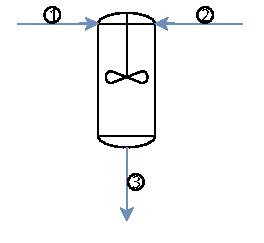
\includegraphics[width=0.55\textwidth]{Diagramas/diagrama/Diagrama_ej15.pdf}
\end{center}

\textit{Paso 2. Tabla de corrientes.}

\begin{center}
\renewcommand{\arraystretch}{1.6}
\begin{tabularx}{\textwidth}{|c|X|X|}
\hline
\textbf{Corriente} & \textbf{$\dot{A}$ (kg/h)} &
\textbf{$\dot{F}$ (kg/h)} \\
\hline
\corriente{1} & 150 & $\dot{F}_1$ \\
\hline
\corriente{2} & 200 & $\dot{F}_2$ \\
\hline
\corriente{3} & $\dot{A}_3$ & $\dot{F}_3$ \\
\hline
\end{tabularx}
\end{center}

\textit{Paso 3. Ecuaciones.}

\textit{Ecuación general.}

\[
\cancelto{0}{\text{Acu}} = \text{Ent} - \text{Sal} + \cancelto{0}{\text{Rx}}
\]

\[
\text{Ent} = \text{Sal}
\]

\textit{Ecuaciones de total.} Como cada corriente es agua pura, el
único componente es el agua ($A$). Entonces el flujo total de cada
corriente coincide con el flujo de agua:
\begin{align*}
\dot{A}_1 &= \dot{F}_1 \\[4pt]
\dot{A}_2 &= \dot{F}_2 \\[4pt]
\dot{A}_3 &= \dot{F}_3
\end{align*}

\textit{Ecuación de balance.} Para el agua, lo que entra es igual a
lo que sale:
\[
\dot{A}_1 + \dot{A}_2 = \dot{A}_3
\]

\textit{Ecuación independiente.} La suma de los flujos totales que
entran es igual a la suma de los que salen:
\[
\dot{F}_1 + \dot{F}_2 = \dot{F}_3
\]

\textit{Paso 4. Resultado.}

Sustituyendo los valores conocidos:
\begin{align*}
\dot{F}_1 &= \dot{A}_1 = 150\,\frac{\mathrm{kg}}{\mathrm{h}} \\[4pt]
\dot{F}_2 &= \dot{A}_2 = 200\,\frac{\mathrm{kg}}{\mathrm{h}} \\[4pt]
\dot{A}_3 &= \dot{A}_1 + \dot{A}_2 = 150 + 200 = 350\,\frac{\mathrm{kg}}{\mathrm{h}} \\[4pt]
\dot{F}_3 &= \dot{A}_3 = 350\,\frac{\mathrm{kg}}{\mathrm{h}}
\end{align*}

\textit{Tabla final.}

\begin{center}
\renewcommand{\arraystretch}{1.6}
\begin{tabularx}{\textwidth}{|c|X|X|}
\hline
\textbf{Corriente} & \textbf{$\dot{A}$ (kg/h)} &
\textbf{$\dot{F}$ (kg/h)} \\
\hline
\corriente{1} & 150 & 150 \\
\hline
\corriente{2} & 200 & 200 \\
\hline
\corriente{3} & 350 & 350 \\
\hline
\end{tabularx}
\end{center}
\end{exercise}

\begin{exercise}{16}{}
Un secador recibe $500\,\mathrm{kg/h}$ de sólido húmedo, compuesto
por sólido y agua. Del secador salen dos corrientes: una de sólido
seco con un flujo de $480\,\mathrm{kg/h}$ y otra de vapor de agua.
Si el secador opera en régimen permanente, ¿cuál es el flujo de la
corriente de vapor?

\textit{Paso 1. DFP del proceso.}

\begin{center}
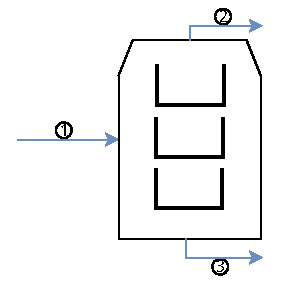
\includegraphics[width=0.55\textwidth]{Diagramas/diagrama/Diagrama_ej16.pdf}
\end{center}

\textit{Paso 2. Tabla de corrientes.}

\begin{center}
\renewcommand{\arraystretch}{1.6}
\begin{tabularx}{\textwidth}{|c|X|X|X|}
\hline
\textbf{Corriente} & \textbf{$\dot{S}$ (kg/h)} &
\textbf{$\dot{A}$ (kg/h)} & \textbf{$\dot{F}$ (kg/h)} \\
\hline
\corriente{1} & $\dot{S}_1$ & $\dot{A}_1$ & 500 \\
\hline
\corriente{2} & $\dot{S}_2$ & $\dot{A}_2$ & 480 \\
\hline
\corriente{3} & $\dot{S}_3$ & $\dot{A}_3$ & $\dot{F}_3$ \\
\hline
\end{tabularx}
\end{center}

\textit{Paso 3. Ecuaciones.}

\textit{Ecuación general.}
\[
\cancelto{0}{\text{Acu}} = \text{Ent} - \text{Sal} + \cancelto{0}{\text{Rx}}
\]
\[
\text{Ent} = \text{Sal}
\]

\textit{Ecuaciones de total.}
\begin{align*}
\dot{S}_1 + \dot{A}_1 &= \dot{F}_1 \\[4pt]
\dot{S}_2 + \dot{A}_2 &= \dot{F}_2 \\[4pt]
\dot{S}_3 + \dot{A}_3 &= \dot{F}_3
\end{align*}

\textit{Ecuaciones de balance.}
\begin{align*}
\dot{S}_1 &= \dot{S}_2 + \dot{S}_3 \\[4pt]
\dot{A}_1 &= \dot{A}_2 + \dot{A}_3
\end{align*}

\textit{Ecuación dependiente.}
\[
\dot{F}_1 = \dot{F}_2 + \dot{F}_3
\]

\textit{Paso 4. Análisis.}

El problema no especifica la composición del sólido húmedo, pero
sí especifica que las corrientes de salida son puras. La corriente
\corriente{2} es sólido seco, así que $\dot{A}_2 = 0$. La corriente
\corriente{3} es vapor de agua, así que $\dot{S}_3 = 0$.

Sustituyendo en las ecuaciones de balance:
\begin{align*}
\dot{S}_1 &= \dot{S}_2 + \cancelto{0}{\dot{S}_3} = \dot{S}_2 \\[4pt]
\dot{A}_1 &= \cancelto{0}{\dot{A}_2} + \dot{A}_3 = \dot{A}_3
\end{align*}

De la ecuación de total para \corriente{2}:
\[
\dot{S}_2 + \cancelto{0}{\dot{A}_2} = 480 \quad \Rightarrow \quad \dot{S}_2 = 480
\]

Como $\dot{S}_1 = \dot{S}_2$, entonces $\dot{S}_1 = 480$.

De la ecuación de total para \corriente{1}:
\[
\dot{S}_1 + \dot{A}_1 = 500 \quad \Rightarrow \quad 480 + \dot{A}_1 = 500
\quad \Rightarrow \quad \dot{A}_1 = 20
\]

Y como $\dot{A}_3 = \dot{A}_1$, entonces $\dot{A}_3 = 20$.

Finalmente, de la ecuación dependiente:
\[
\dot{F}_3 = \dot{F}_1 - \dot{F}_2 = 500 - 480 = 20\,\frac{\mathrm{kg}}{\mathrm{h}}
\]

\textit{Paso 5. Resultado.}

Sustituyendo los valores:
\begin{align*}
\dot{S}_1 &= 480\,\frac{\mathrm{kg}}{\mathrm{h}} \\
\dot{A}_1 &= 20\,\frac{\mathrm{kg}}{\mathrm{h}} \\
\dot{F}_1 &= 500\,\frac{\mathrm{kg}}{\mathrm{h}} \\[4pt]
\dot{S}_2 &= 480\,\frac{\mathrm{kg}}{\mathrm{h}} \\
\dot{A}_2 &= 0\,\frac{\mathrm{kg}}{\mathrm{h}} \\
\dot{F}_2 &= 480\,\frac{\mathrm{kg}}{\mathrm{h}} \\[4pt]
\dot{S}_3 &= 0\,\frac{\mathrm{kg}}{\mathrm{h}} \\
\dot{A}_3 &= 20\,\frac{\mathrm{kg}}{\mathrm{h}} \\
\dot{F}_3 &= 20\,\frac{\mathrm{kg}}{\mathrm{h}}
\end{align*}

\textit{Tabla final.}

\begin{center}
\renewcommand{\arraystretch}{1.6}
\begin{tabularx}{\textwidth}{|c|X|X|X|}
\hline
\textbf{Corriente} & \textbf{$\dot{S}$ (kg/h)} &
\textbf{$\dot{A}$ (kg/h)} & \textbf{$\dot{F}$ (kg/h)} \\
\hline
\corriente{1} & 480 & 20 & 500 \\
\hline
\corriente{2} & 480 & 0 & 480 \\
\corriente{3} & 0 & 20 & 20 \\
\hline
\end{tabularx}
\end{center}
\end{exercise}

\begin{notaimportante}
\textbf{Sobre cómo se descompone una mezcla.} Una corriente que
contiene varios componentes (como un sólido húmedo: sólido + agua)
no se trata como un solo compuesto. Se descompone en sus
componentes desde el inicio, y cada componente se balancea por
separado. Si se trata como un solo compuesto, aparece la tentación
de escribir una ``transformación'' de un compuesto en otros
(como $\dot{S_h}_1 \to \dot{S}_2 + \dot{A}_3$), pero eso no es
una reacción química: es una separación física. En una separación,
ningún componente se genera ni se consume, solo se redistribuye
entre las corrientes de salida.

Esto es la diferencia entre el ejercicio 16 (sólido húmedo) y el
ejercicio 8 del temario (evaporador de jarabe). En el evaporador,
el enunciado dice desde el inicio qué fracción es sólido y qué
fracción es agua, y los balances se plantean por componente sin
dificultad. En el ejercicio 16, si el enunciado no especifica la
composición del sólido húmedo, hay que deducirla del balance
mismo. Pero nunca se trata como si fuera un compuesto único.
\end{notaimportante}

\begin{notafija}
\textbf{Reglas visuales de las tablas.} Las tablas de flujos y las de
composición se leen distinto:

\begin{itemize}
    \item \textbf{Tabla de flujos por componente:} las sumas
    \textbf{horizontales} dan el flujo total de cada corriente
    ($\dot{A}_i + \dot{B}_i + \dot{C}_i = \dot{F}_i$). Las sumas
    \textbf{verticales} dan el balance por componente
    ($\sum \dot{A}_{\text{entrada}} = \sum \dot{A}_{\text{salida}}$).
    Las dos sumas tienen significado físico.

    \item \textbf{Tabla de composición:} solo las sumas
    \textbf{horizontales} tienen significado. Cada renglón suma 1
    ($w_i^A + w_i^B + w_i^C = 1$). Las sumas verticales no tienen
    sentido: no se suman fracciones del mismo componente en
    distintas corrientes.

    \item \textbf{Relación entre las dos tablas:} el flujo de un
    componente se obtiene multiplicando su composición por el flujo
    total de la corriente:
    \[
    \dot{J}_i = w_i^J \cdot \dot{F}_i
    \qquad \text{o} \qquad
    \dot{J}_i = \chi_i^J \cdot \dot{F}_i
    \]
    según se trabaje en masa o en mol.
\end{itemize}
\end{notafija}

prueba